\appendix

\setcounter{chapter}{0}

\part{Appendix}

In this part, we are going to deal with the organization of the team on this project. First, we identified the different tasks which will constitute this project. Thanks to elements identified previously, we made a Gantt diagram which is a tool used in project management, and allowing the affectation of a task for one person or a group of person, the time which this task will have to take. He allows to visualize the fulfillment of the tasks according to time.

\chapter{Requirements}

\section{Functional Requirements}

\begin{itemize}

\item The area coverage\\
We need to cover the area the most efficiently and rapidly.

\item The connectivity\\
UAVs need to be always in contact with the C\&C to transmit the information at any time.

\end{itemize}

\section{Non-Functional Requirements}

\begin{itemize}

\item No excessive use of bandwidth\\
The bandwidth is a limited and a precious resource. Therefore UAVs have to used bandwidth the better possible to not overloaded her.

\item Regurlarly updated the information\\
UAVs transmit their information to the C\&C and other UAVs when they are near . Thus, if a UAV have data much old, it is possible that he scans a part of the area already scanned. Hence, the data transmitted by UAVs have not to be older than prescribed and if each UAV has up-to-date information, the scan coverage will be more quickly.

\item A robust model\\
Lost or unaivable UAVs during a scenario not involved the good progress of the scan coverage. The resulting of a lost UAV should not degrade the final result.

\end{itemize}

\chapter{Architecture}

\subsubsection{Random Model}

\begin{figure}[!h]
\center
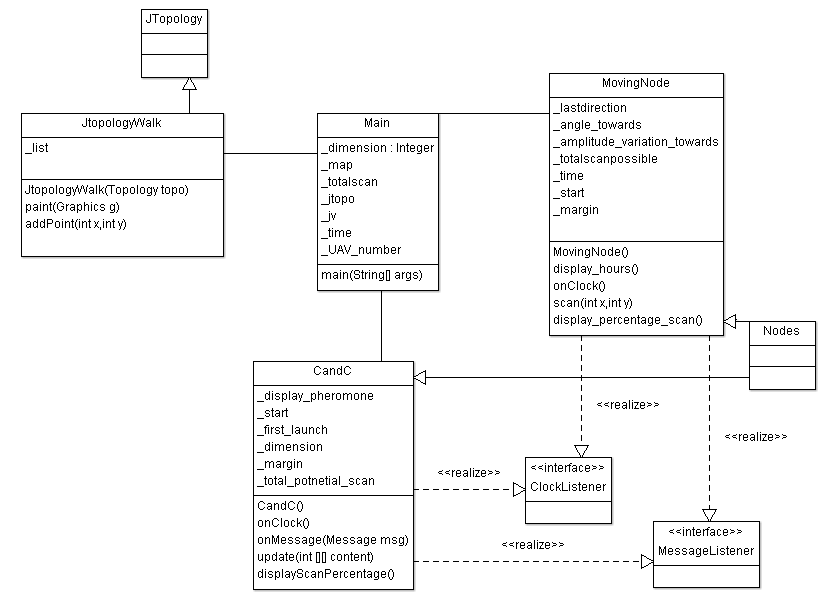
\includegraphics[scale=0.7]{../images/DiagrammedeclassesRandom.png}
\caption{\label{RandomWalkDIA}Diagram of class Random model}
\end{figure}

\newpage

\subsubsection{Pheromone model}

\begin{figure}[!h]
\centering
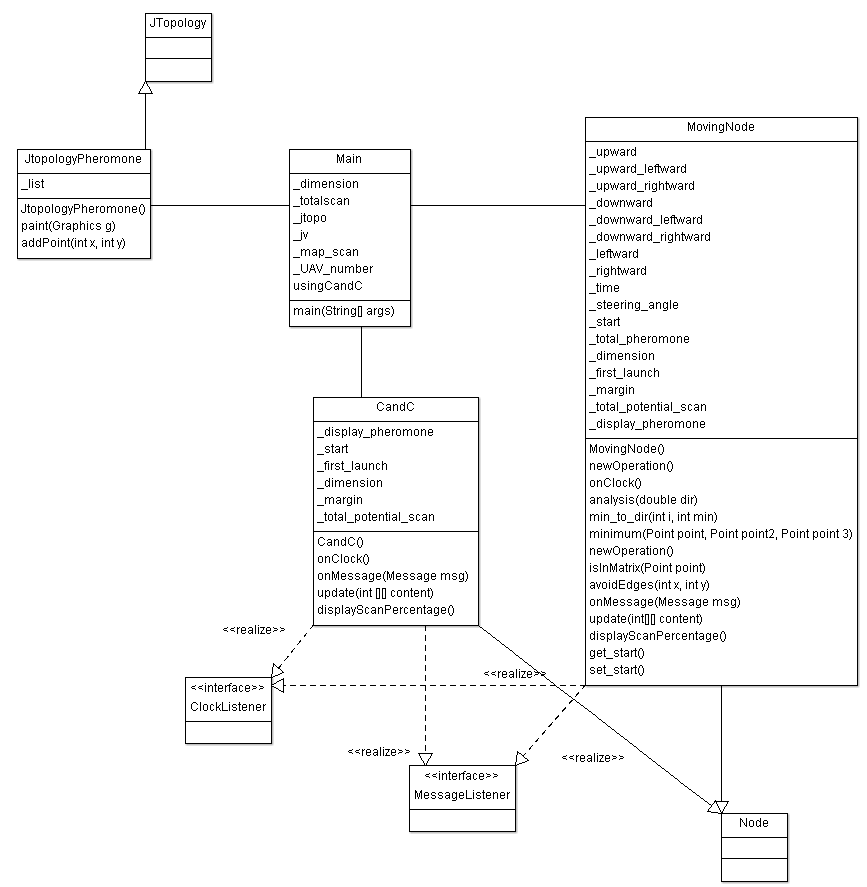
\includegraphics[scale=0.6]{../images/DiagrammedeclassesPheromone.png}
\caption{\label{RandomWalkDIA}Diagram of class Pheromone model}
\end{figure}

\chapter{Schedule}

\section{Tasks list}

A list of task was identified from the beginning by the project to be able to lead it most effectively possible from the beginning to the end.

\begin{itemize}
\item The choice of the subject. We took a subject which concerned drones because the majority of our team follow the subject Communicating Autonomous Systems.
\item An analysis of existing concerning the communicating autonomous systems. We read about ten articles in touch with our main subject.
\item An update of various articles previously studied is essential. Indeed, the speed of evolution of the technology today is so important that a written article two or three years ago may be out of date.
\item The development of both present models in the studied article.
\item The writing of this report.
\item The preparation of the orals.
\end{itemize}

\newpage

\section{GANTT}

\begin{figure}[htbf]
\center
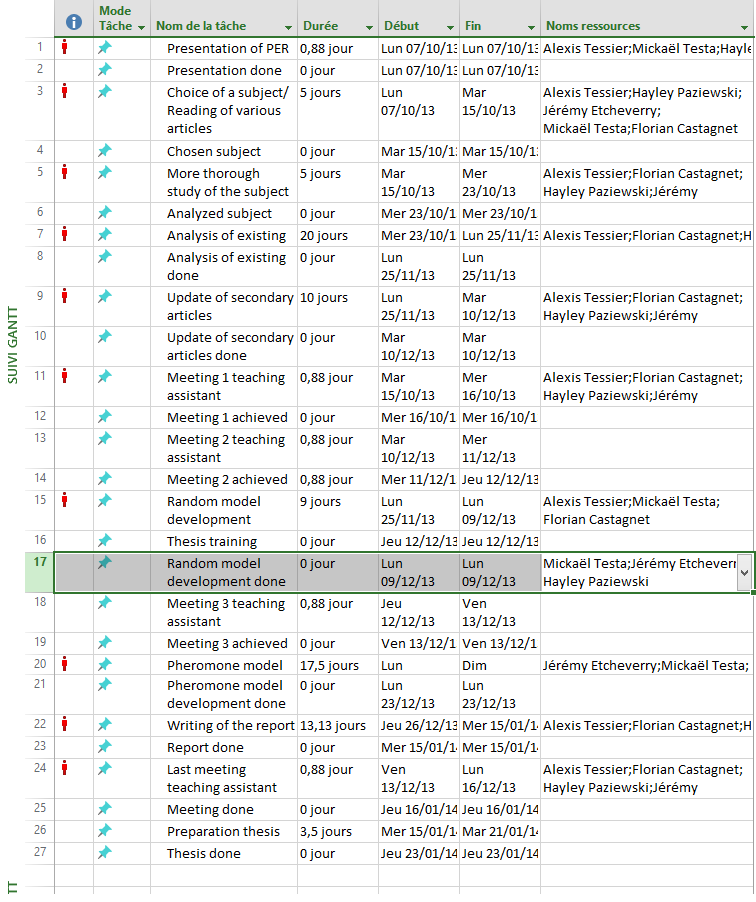
\includegraphics[scale=0.7]{../images/Gantt1.png}
\caption{\label{Gantt}Diagram of Gantt of our project}
\end{figure}

\newpage

\begin{figure}[htbf]
\center
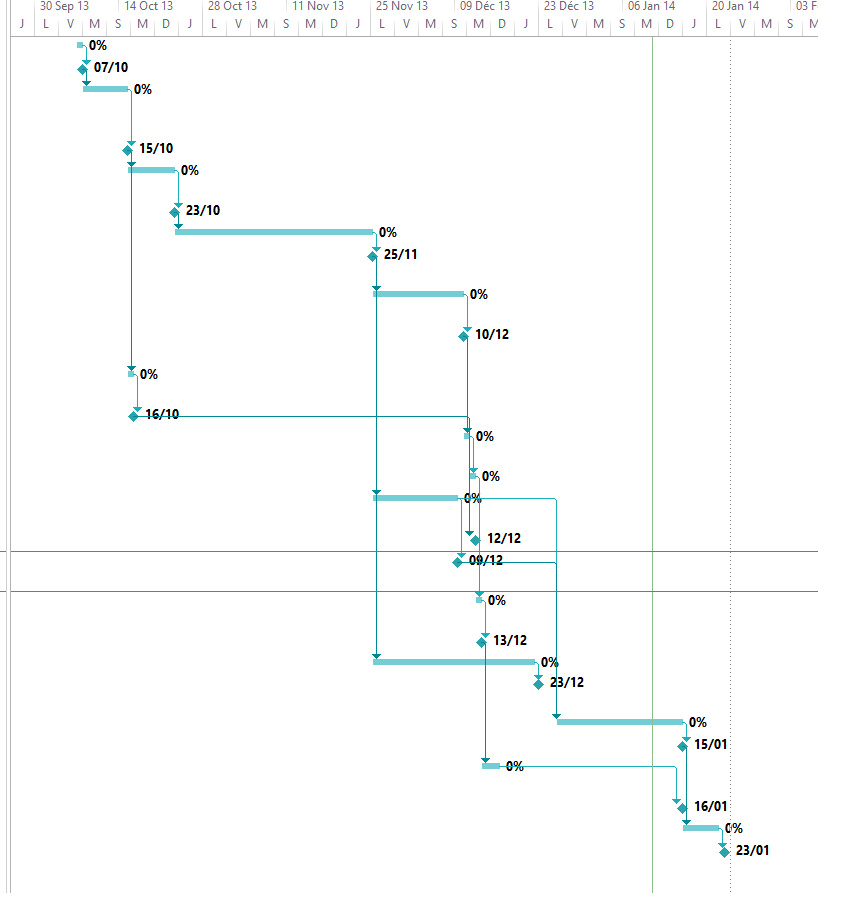
\includegraphics[scale=0.7]{../images/Gantt2.png}
\caption{\label{Gantt}Diagram of Gantt of our project}
\end{figure}

\chapter{Development environment and conventions}

\section{Development environment}

\subsection{GitHub}

To write this report and to be able to implement both models most effectively possible, we used a tool of hosting and management of program which is called Github. It is a tools of versionning which allows the collaborative work and allows a simplification of the methods of work.\\

We used it throughout the project to put the summaries of articles that we read, the result og our meeting, this report or still implementations.\\
Our Git repository is located at the following address : \\
\url{https://github.com/jetcheve/M2\_PER\_MMUAVGRA}.\\

\noindent Our deposit is decomposes into three branches :

\begin{itemize}
\item A master branch which is general to the whole deposit.
\item A branch called Develop. It's in this branch that there will be all the code for implementing different models.
\item An branch report, which as its name suggests, contain all the parts of our report and his pictures.
\end{itemize}

\subsection{Eclipse}

Eclipse is an integrated development environment for creating projects in any programming language. It is used to develop programs in JAVA, Android, C, etc.\\

\noindent We used Eclipse throughout the project implementation.\\

As a supplement to Eclipse, we used a library that is called JBotsim \cite{JBotSim} proposed by Mr. Casteigts. This allows to simulate a dynamic network. This network is simulated with mobile nodes that interact. These nodes can send messages (in our case, maps of each UAVs).\\

We used this library because it is very easy to use, and it adapt well to the needs which we had.

\section{Programming Conventions}

First, we've choosed to used the Java Coding Conventions, which we can see in the following link \url{http://www.oracle.com/technetwork/java/codeconventions-150003.pdf}\\

Then, in order to create our documentation, we've used the Doxygen Convention, viewable here \url{http://www.stack.nl/~dimitri/doxygen/manual/docblocks.html}\\
We've relied heavily on this documentation and have mostly employed these protocoles below.\\

\lstset{language=Java,basicstyle=\footnotesize,commentstyle=\color{blue}}
\begin{lstlisting}[frame=trBL, title=Doxygen Convention for classes]
/**
* @class name of the class
* @brief Description of herself
*/
\end{lstlisting}

\lstset{language=Java,basicstyle=\footnotesize,commentstyle=\color{blue}}
\begin{lstlisting}[frame=trBL, title=Doxygen Convention for methods]
/**
* @brief Description of the method
* @param the parameters and their descriptions
* @return the description of what return the method (optional)
*/
\end{lstlisting}

\lstset{language=Java,basicstyle=\footnotesize,keywordstyle=\color{red},commentstyle=\color{blue}}
\begin{lstlisting}[frame=trBL, title=Doxygen Convention for members]
int _var; /**< Detailed description after the member */
\end{lstlisting}
~\\

We've also resorted to programming conventions that we defined between us.\\
For example, we put all of our functions names or variable names, in the same language (English).\\

Then, when a part of a code, was not finished yet, we put the following lines above the concerning part.

\lstset{language=Java,basicstyle=\footnotesize,commentstyle=\color{blue}}
\begin{lstlisting}[frame=trBL, title=Programming convention for unfinished code]
/**
* @TO_DO
* Description
*/
\end{lstlisting}
~\\

We've also used a convention for the bugs found and wrote these lines.\\

\lstset{language=Java,basicstyle=\footnotesize,commentstyle=\color{blue}}
\begin{lstlisting}[frame=trBL, title=Programming convention for bugs]
/**
* @BUG
* Description
*/
\end{lstlisting}
~\\

\noindent We've used GitHub too, in order to manage us. Indeed, it allows us :

\begin{itemize}
\item to create tasks, 
\item assign somebody to a task, 
\item see if a task is finish or not,
\item create Milestones, which is a set of tasks to do in a specific time, 
\item and see the state of our progress,
\item define kinds of tasks (development, bug, report ...)
\end{itemize}

\newpage

\begin{figure}[!h]
   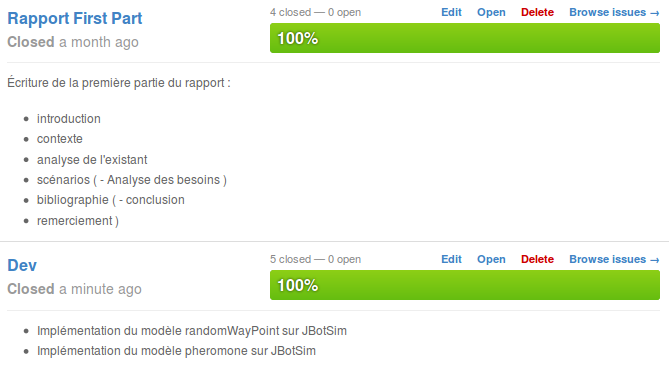
\includegraphics[scale=0.7]{../images/Milestones.png}
\caption{\label{Milestones}Progress state of Milestones}
\end{figure}

\begin{figure}[!h]
\center
   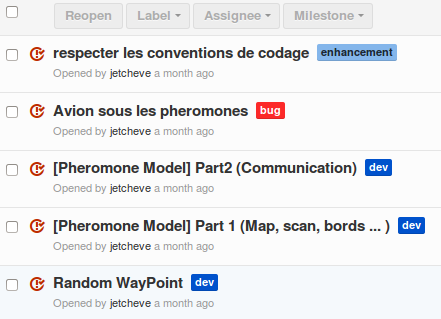
\includegraphics[scale=0.7]{../images/tasks.png}
\caption{\label{Tasks}Example of Tasks}
\end{figure}

\newpage

To finish, we've created the five essential files for a project :

\begin{itemize}
\item INSTALL.txt  : Installation instructions for the project,
\item LICENCE.txt  : Licence and copyright \copyright{} of the project,
\item README.txt   : General description of the project,
\item AUTHORS.txt  : Authors of the project,
\item MANIFEST.txt : Tree structure and files list of the project.
\end{itemize}